\documentclass[]{article}
\usepackage{natbib}
\usepackage[margin=0.5in]{geometry}

\usepackage[FIGTOPCAP,tight]{subfigure}
\usepackage{graphicx}
\usepackage{hyperref}
\usepackage{amsmath}


%opening
\title{Differential Chromatic Refraction: literature overview}
\author{I. S. Sullivan, D. J. Reiss}

\begin{document}

\maketitle


%\begin{abstract}
%
%\end{abstract}

\section{Overview}
Like any medium, the Earth's atmosphere refracts incident light, which for an observer on the Earth's surface results in a deflection of the apparent position of sources towards zenith by about 1 arcsecond per degree of the source from zenith. This bulk effect of refraction is well understood in astronomical applications and is easily accounted for most of the optical through radio wavelengths where the index of refraction is constant, but towards the blue end of the optical spectrum atmospheric dispersion results in increasing refraction. As a result, photons from the same source but different wavelengths that pass through the same filter of a telescope will have slightly different degrees of refraction and will land on different locations of the detector, an effect called Differential Chromatic Refraction (DCR). Differential Chromatic Refraction was first raised as an issue for spectrometry in \cite{Filippenko1982}, where the problem was framed as a loss of flux in slit spectrometers. The issue has now become important for imaging cameras as well, though, because high-resolution cameras such as the LSST will experience significant PSF smearing in the u and g bands (Figure  \ref{Fig:DCR-wavelength-ZA}).


\begin{figure*}
	\begin{center}
		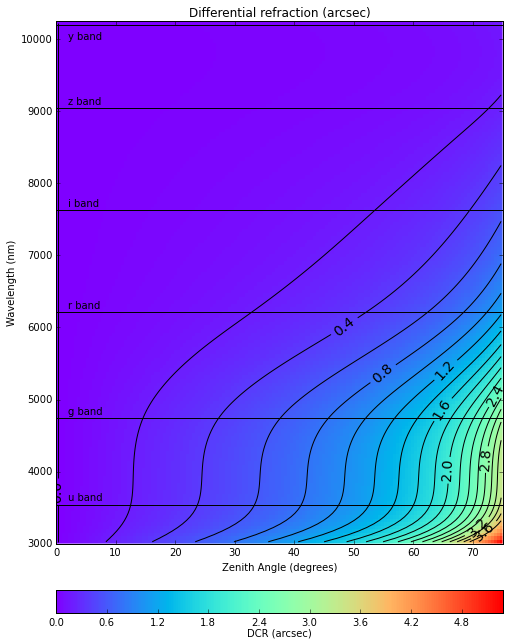
\includegraphics[height=9in]{DCR_ZA-wavelength}
		\caption{Maximum DCR over a range of zenith angles and wavelengths. Each wavelength is treated as the center wavelength of a band with 20\% bandwidth, and maximum DCR is calculated for the difference in position of two photons from the same source at opposite ends of the band.}
		\label{Fig:DCR-wavelength-ZA}
\end{center}
\end{figure*}
\begin{figure*}
	\begin{center}
		\subfigure[Pressure and Temperature]{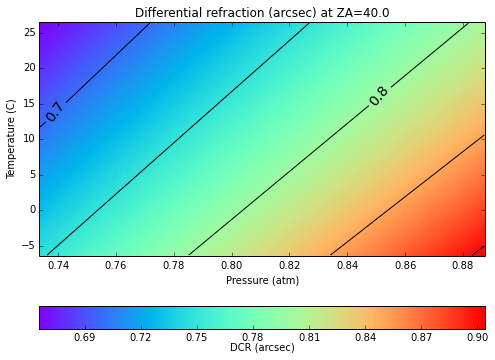
\includegraphics[height=2.8in]{DCR_Pressure-Temperature}}
		\subfigure[Zenith Angle and Pressure]{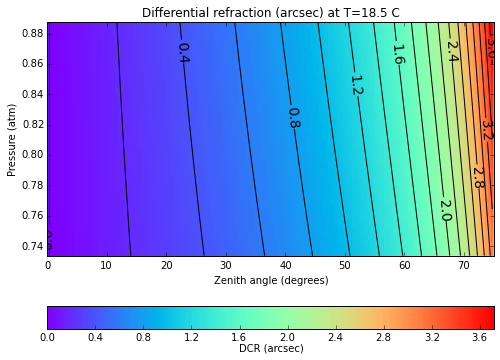
\includegraphics[height=2.8in]{DCR_ZA-Pressure}}
		\subfigure[Zenith Angle and Temperature]{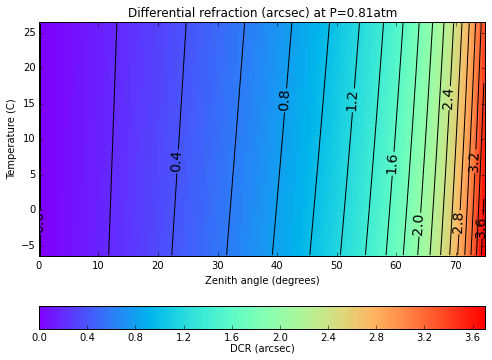
\includegraphics[height=2.8in]{DCR_ZA-Temperature}}
		\caption{Investigation of maximum DCR under varying conditions for LSST u' band. For a given filter, maximum DCR depends on the zenith angle of observation (airmass), atmospheric pressure, temperature, and, to a lessor degree, humidity. In panels (a) - (c) we keep one of the three main parameters fixed at a nominal value, and map the full range of realistic observing conditions for the remaining two to get a feel for the relative importance of each.}
		\label{Fig:DCR-P-T}
	\end{center}
\end{figure*}

\section{DCR literature}
A quick summary of and notes on the existing literature covering DCR. Each reference we found is covered in it's own subsection below.

\subsection{Report on Summer 2014 Production: Analysis of DCR (Andrew Becker)}

\url{https://github.com/lsst-dm/S14DCR/blob/master/report/S14report_V0-00.pdf}

\begin{itemize}
	\item Estimated DCR effects directly for LSST using catSim's stellar
	SEDs.
	\item Investigated only airmass effects (no temperature,
          etc. dependence).
	\item Utilized 5 mas threshold for "good" DCR corrections
          based on estimated accuracy required for difference imaging
          (no dipoles).
	\item Summmary of DCR estimates:
	
	\begin{itemize}
		
		\item For \textit{g} and \textit{r}, nearly all stars
                  will exhibit differential DCR of $>$ 5 mas at
                  parallactic angle differences $>$ 20 deg. or airmass
                  differences of $>$ 0.15.
		\item For \textit{i}, similar effects for parallactic
                  angle differences $>$ 25 deg. or airmass differences
                  $>$ 0.2, mostly for M-dwarf stars.
		\item For \textit{z}, only very large differences in
                  parallactic angle or airmass lead to DCR $>$ 5 mas.
	\end{itemize}
	\item DCR corrections tested based on modeling using colors and airmass terms.
	\begin{itemize}
		\item Random forest regression models provided most
                  accurate modeling of DCR and refraction.
		\item \textit{u} and \textit{g} models worked but
                  would be degraded by 10\% color errors (\textit{u})
                  or 2.5\% color errors (\textit{g}).
		\item \textit{riz} models could correct all but
                  $10^{-5}$ stars to $<$ 5 mas residuals.
	\end{itemize}
\end{itemize}

**Recommendations**:
\begin{itemize}
	\item Code from the S14DCR analysis
          \url{https://github.com/lsst-dm/S14DCR} should be updated to
          use latest version of sims\_photUtils and include estimates
          for galaxies and SNe.
%	\item Potentially merge capabilities of SED and Bandpass in sims\_photUtils with those from chroma \url{https://github.com/DarkEnergyScienceCollaboration/chroma/}; see below.
	\item Understand how DCR calcs are performed in sims pipeline
          to compare the results of these simulations to DCR effects
          in simulated images, and to enable investigation of DCR
          corrections on image coadds and differences (see also
          \url{https://github.com/lsst-dm/W14ImageDifferencing}).
\end{itemize}


\begin{figure}[t!]
	\begin{center}
		\subfigure[Difference image with no DCR correction]{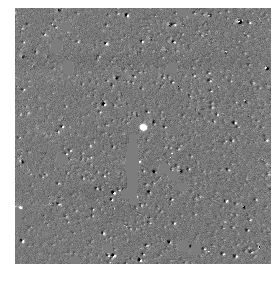
\includegraphics[height=2.8in]{9903215v1_f5a.png}}
		\subfigure[Difference image with DCR correction]{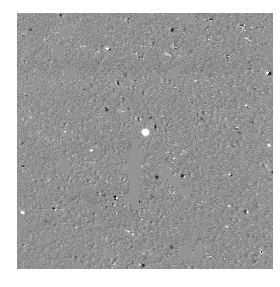
\includegraphics[height=2.8in]{9903215v1_f5b.png}}
		\caption{(\citeauthor{AlcockDiffIm1999} Fig. 5.)— "The effect of differential refraction on difference images. Left image is a difference image without applying any correction for differential refraction effects. The right image is the same image with our correction technique applied. The scale of the noise structures is much reduced although not completely removed. The two images are 100′′ ×100′′. The residual object in the centre is due to a variable star"}
		\label{Fig:Alcock5}
	\end{center}
\end{figure}


\subsection{\cite{AlcockDiffIm1999}}
\begin{itemize}
	\item Investigation of DiffIm for MaCHO search.
	\item This is the only reference I could find that described a method
	to correct for DCR for image differencing. Suggestion is to compute a
	per-pixel color map of each field (using images near zenith or at
	least at the same airmass and parallactic angle). They then
	interpolated the pixel values in the template image based on the
	color map pixel values, the airmass of the observation relative to
	the reference image, and the parallactic angle of the observation.
	\item Improvements were obtained by differencing a number of images
	taken at a range of airmasses to obtain a semi-empirical result for
	the offset required with color and airmass (relative to the
	reference image).
	\item The results shown in Figure \ref{Fig:Alcock5} suggest moderate success with this
	strategy.
\end{itemize}

\subsection{\cite{Hohenkerk1985}}
\begin{itemize}
	\item Good background.
	\item Uses a different implementation, "the method recommended by Auer
	and Standish".
	\item This is the function implemented in `pypal` which is used by
	some (but not all?) code in the `sims` stack.
	\item Uses a model atmosphere with temperature and pressure gradients,
	integrated to the surface.  This I believe is different from \cite{Filippenko1982}
	which assumes a single refractive surface.
\end{itemize}

\subsection{\cite{Meyers2015}}

\begin{itemize}
	\item Estimates of DCR on weak lensing measurements.
	\item Source code for analysis is available here:
          \url{https://github.com/DarkEnergyScienceCollaboration/chroma/}.
	\item Primarily measured effects of DCR on shape measurements
          (2nd moments); code can be used to estimate 1st moments for
          a given SED. Preliminary code:
          \url{https://github.com/isullivan/LSST-DCR/tree/master/code/notebooks}.
        \item Also investigated effects of 1st moments for galaxy SEDs
          and compensation via extra trees regression on LSST colors.
\end{itemize}

%**Recommendations**:
%\begin{itemize}
%	\item Check and incorporate DCR code from their chroma package into sims pipelines
%\end{itemize}

\subsection{\cite{Chambers2005}}

\begin{itemize}
	\item Updated summary of (more accurate?) astrometric transformations including DCR.
	\item Estimated astrometric accuracy in Pann-STARRS of 1
          mas. This assumes accurate atmospheric characterization for
          each field from sky probes (atmospheric absorption).
\end{itemize}

**Recommendations**:
\begin{itemize}
	\item Understand these transformations. Suggestion is that C
          code exits somewhere in the Pan-STARRS codebase, but I could
          not find it.
\end{itemize}

\subsection{\cite{AlejandroPlazas2012}}
\begin{itemize}
	\item Investigates the effect of DCR on weak lensing measurements through the second moment of galaxy shape measurements.
	\item Finds that "Using standard galaxy and stellar spectral templates we calculate the resultant errors in the griz bands, and find that atmospheric dispersion shear systematics, left uncorrected, are up to 6 and 2 times larger in g and r bands, respectively, than the thresholds at which they become significant contributors to the DES error budget, but can be safely ignored in i and z bands. For the stricter \textit{LSST} requirements, the factors are about 30, 10, and 3 in g, r, and i bands, respectively"
\end{itemize}

\subsection{\cite{Stone1996}}
\begin{itemize}
	\item A good reference giving equations for refraction
          including the effect of temperature, pressure, and water
          vapor pressure. Used for calculating Figure
          \ref{Fig:DCR-P-T}
          We summarize the environmental and observing condition parameters in Table \ref{table:parameters} and list the units and range of validity for the equations for each.

\end{itemize}

\begin{table}[h!]
	\begin{center}
	\begin{tabular}{c | c | c | c}
		Parameter & valid range & description & units \\
		\hline
		$P_s$& $0$ mbar$ < P_s < 4000$ mbar & Atmospheric pressure & millibar  \\
		$RH$ & $0\% < RH < 100\%$ & Relative humidity & Percent \\
		$\lambda$& $2302$\AA{}$ < \lambda < 20,586 $\AA{} & Wavelength  & Angstroms \\
		$T$& $250K < T < 320K$ & Temperature & Kelvin \\
		$\phi$ & $0^\circ \leq \phi < 360^\circ$ & Latitude of the observing site & Degrees \\
		$h$ & $0\,m\leq h$ & Elevation of the observing site & meters \\
		$z_0$ & $0^\circ\leq z_0 < 75^\circ$ & Zenith angle & Degrees
		
	\end{tabular}
	\end{center}
	\caption{Definition of parameters and their units}
	\label{table:parameters}
\end{table}
%\vspace{-0.7cm}

The refraction of monochromatic light is given by
\begin{align}
R(\lambda) &= r_0 n_0(\lambda) \sin z_0 \int_1^{n_0(\lambda)} \frac{dn}{n \left(r^2n^2 -r_0^2n_0(\lambda)^2\sin^2z_0\right)^{1/2}} \nonumber\\
&\simeq \kappa (n_0(\lambda) - 1) (1 - \beta) \tan z_0 - \kappa (1 - n_0(\lambda)) \left(\beta - \frac{n_0(\lambda) - 1}{2}\right) \tan^3z_0
\end{align}
where $n_0(\lambda)$, $\kappa$, and $\beta$ are given by equations \ref{eqn:index_refraction}, \ref{eqn:kappa}, and \ref{eqn:beta} below, respectively.

To calculate refraction, we need to know the local index of refraction of air $n_0(\lambda)$ at the observatory site:
\begin{align}
	n_0(\lambda) =&1 + \left(\left[2371.34 +\frac{683939.7}{130 - \sigma(\lambda)} +\frac{4547.3}{38.9 - \sigma(\lambda)^2}\right] D_s 
		+ \left(6487.31 + 58.058 \sigma(\lambda)^2 - 0.71150 \sigma(\lambda)^4 +0.08851 \sigma(\lambda)^6\right) D_w \right)\times 10^{-8} \label{eqn:index_refraction}\\*
	& where \nonumber\\*
	\sigma(\lambda) &= 10^4 /\lambda \;\;\;\;\left(\mu m^{-1}\right)\nonumber \\*
	D_s =& \left[1 + (P_s-P_w) \left(57.90\times10^{-8} - \frac{9.3250\times10^{-4}}{T}+\frac{0.25844}{T^2}\right)\right] \frac{(P_s-P_w)}{T} \nonumber \\*
	D_w =& \left[1 + P_w \left(1 + 3.7\times10^{-4} P_w\right)\left(-2.37321\times10^{-3} + \frac{2.23366}{T} - \frac{710.792}{T^2} + \frac{7.75141\times10^4}{T^3}\right)\right] \frac{P_w}{T} \nonumber \\
	P_w =& RH\times 10^{-4} \times e^{(77.3450 + 0.0057 T - 7235.0/T)}/T^{8.2} \nonumber
\end{align}

where the parameters $D_s$ and $D_w$ are the density factors for dry air and water vapor, respectively, taken from \cite{Owens:67}.

The ratio of local gravity at the observing site to $g = 9.81 m/s^2$ is given by
\begin{equation}
\kappa = g_0/g = 1 + 5.302\times 10^{-3} \sin^2\phi - 5.83\times 10^{-6} \sin^2(2\phi) - 3.15\times 10^{-7} h \label{eqn:kappa}
\end{equation}

If we assume an exponential density profile for the atmosphere, then the ratio $\beta$ of the scale height of the atmosphere to radius of the observing site from the Earth's core can be approximated by:
\begin{align}
	\beta &= \frac{1}{R_\oplus}\int_{0}^\infty \frac{\rho}{\rho_0} dh \nonumber \\
	&\simeq \frac{P_s}{\rho_0g_0 R_\oplus} = \frac{k_BT}{m g_0 R_\oplus} \nonumber \\
	&=  4.5908\times 10^{-6} T \label{eqn:beta}
\end{align}
where $m$ is the average mass of molecules in the atmosphere, $R_\oplus$ is the radius of the Earth, $k_B$ is the Boltzmann constant, and $g_0$ is the acceleration due to gravity at the Earth's surface.



\subsection{\cite{Filippenko1982}}
\begin{itemize}
	\item Original paper posing DCR as a problem to be addressed. Mostly of historical interest.
	\item Focused on the effect on spectrometers, with the
	recommendation that slit spectrometers be aligned with fixed
	parallactic angle. 
\end{itemize}

\subsection{\cite{Cuby1998}}
\begin{itemize}
	\item As with \citeauthor{Filippenko1982}, concerned with flux loss in slit spectrometers. 
	\item Discusses observing strategies for spectrometers to keep flux loss $< 20\%$ at $z_0<50^\circ$
\end{itemize}
\bibliographystyle{apalike}
\bibliography{DCR_references}


\end{document}


